% Insert after the existing appendices; do not issue another \appendix.
% Requires amsmath, amssymb, graphicx, and booktabs.
% Figure paths are relative to the manuscript root containing figs/.
% Uses the notation of Appendix app:fsm_innovation_energy.

\section{Population objective and empirical estimation bias}
\label{app:ws_bias_analysis}

\subsection{Population-objective identities}
\label{app:ws_bias_population}

The following identities concern fixed candidate parameters and stationary
signals with the displayed second moments finite, under the
input--innovation independence and model assumptions of
Appendix~\ref{app:fsm_innovation_energy}.
Write $\delta\theta=\theta-\theta^\star$.

\paragraph{PL parametrization.}
Let $\varphi^\star(t)^\top$ denote the ideal PL regressor row formed with
the true internal signal $\alpha^\star$, the measured input, and past
true disturbances $e^\star$, using the adopted normalization. The system
equations give
\begin{equation}
\label{eq:bias_PL_true_regression}
 c(t)=\varphi^\star(t)^\top\theta^\star+\nu(t),
 \qquad
 \mathbb E[\varphi^\star(t)\nu(t)]=0.
\end{equation}
The orthogonality follows because the signal-path entries are functions
of the input, which is independent of the innovation process, while the
disturbance-path entries involve past disturbances. Thus, defining
$\Gamma_\varphi=\mathbb E[\varphi^\star(t)\varphi^\star(t)^\top]$, the
ideal population objective satisfies
\begin{equation}
\label{eq:bias_population_PL}
 2\mathcal J_{\mathrm{PL}}^\star(\theta)
 :=\mathbb E[(c(t)-\varphi^\star(t)^\top\theta)^2]
 =\sigma_\nu^2+\delta\theta^\top\Gamma_\varphi\delta\theta.
\end{equation}
Indeed, the residual is
$\nu(t)-\varphi^\star(t)^\top\delta\theta$, and the cross term
vanishes by \eqref{eq:bias_PL_true_regression}.
If $\Gamma_\varphi\succ0$, the unique minimizer is $\theta^\star$.
This is the usual innovation-regression argument underlying classical
PL identification theory \cite{LjungSoderstrom1983}.

The implemented PL criterion instead freezes a reconstructed row
$\hat\varphi^{(k)}(t)^\top$ of $\hat\Phi^{(k)}$ during an inner update.
To state its population identity without assuming perfect reconstruction,
fix a row index $t$ and define the following moments whenever they exist
(their dependence on $t$ is suppressed):
\begin{align}
\label{eq:bias_PL_reconstruction}
 \varepsilon^{(k)}(t)
 &=\nu(t)+[\varphi^\star(t)-\hat\varphi^{(k)}(t)]^\top\theta^\star,\\
 R_k&=\mathbb E[\hat\varphi^{(k)}(t)\hat\varphi^{(k)}(t)^\top],
 \qquad
 q_k=\mathbb E[\hat\varphi^{(k)}(t)\varepsilon^{(k)}(t)].\nonumber
\end{align}
For
$\mathcal J_{\mathrm{PL}}^{(k)}(\theta)
=\frac12\mathbb E[(c(t)-\hat\varphi^{(k)}(t)^\top\theta)^2]$,
expanding the square yields the exact quadratic identity
\begin{equation}
\label{eq:bias_population_PL_reconstructed}
 2\mathcal J_{\mathrm{PL}}^{(k)}(\theta)
 =\mathbb E[(\varepsilon^{(k)}(t))^2]
  -2\delta\theta^\top q_k+\delta\theta^\top R_k\delta\theta.
\end{equation}
The expected record-averaged criterion has the same form, with the
moments averaged over the retained time indices.
If $R_k\succ0$, its unconstrained population minimizer is
$\theta^\star+R_k^{-1}q_k$. Consequently, the practical PL surrogate
is minimized at the truth when $q_k=0$; ideal reconstruction is a
sufficient condition, but joint estimation alone neither guarantees
nor violates this orthogonality. The shift $R_k^{-1}q_k$ describes
the minimizer of a frozen population surrogate, not the finite-record
bias of the complete iterative algorithm. Its evolution across outer
iterations requires a separate convergence analysis.

\paragraph{FSM parametrization.}
For the direct innovation criterion, define
\begin{align}
\label{eq:bias_population_objective}
 \mathcal J_{\mathrm{FSM}}(\theta)
 &=\frac12\mathbb E[r_{\nu,\mathrm{FSM}}^2(t;\theta)],\\
\label{eq:bias_population_definitions}
 \Delta\beta(t;\theta)
 &=\beta_{\mathrm{FSM}}(t;\theta^\star)
       -\beta_{\mathrm{FSM}}(t;\theta),\\
 d&=[d_1,\ldots,d_{n_d}]^\top,\qquad
 E^\star(t)=[e^\star(t-1),\ldots,e^\star(t-n_d)]^\top,\nonumber\\
 \Gamma_e&=\mathbb E[E^\star(t)E^\star(t)^\top].\nonumber
\end{align}
For an exact signal representation, the residual decomposition in
Appendix~\ref{app:fsm_innovation_energy} gives
\[
 r_{\nu,\mathrm{FSM}}(t;\theta)
 =\nu(t)+(d-d^\star)^\top E^\star(t)
       +D(z^{-1};\theta)\Delta\beta(t;\theta).
\]
The cross terms vanish by input--innovation independence and
orthogonality of the current innovation to past disturbances. Hence
\begin{equation}
\label{eq:bias_population_identity}
 2\mathcal J_{\mathrm{FSM}}(\theta)
 =\sigma_\nu^2
  +(d-d^\star)^\top\Gamma_e(d-d^\star)
  +\mathbb E\!\left[
    \left(D(z^{-1};\theta)\Delta\beta(t;\theta)\right)^2\right].
\end{equation}
With $\Gamma_e\succ0$ and an identifiable normalized signal
parametrization, $\theta^\star$ uniquely minimizes this ideal
population objective.

For a finite FSM approximation, $\Delta\beta$ must instead denote the
true deterministic signal minus $\beta_{\mathrm{FSM}}(t;\theta)$.
The identity retains its form, but this mismatch need not vanish at
the physical parameter $\theta^\star$. Thus the practical PL analysis
must account for regressor reconstruction, whereas the FSM analysis
must account for its finite signal representation. Both also require
consistent treatment of finite-record initial states. Neither ideal
population identity, by itself, establishes finite-record unbiasedness.

\subsection{Scope of an analytical bias expression}
\label{app:ws_bias_algorithm}

PL identification has a substantial analytical literature. Classical
work studies convergence points and local and global convergence of
recursive least-squares, generalized and extended least-squares, and
maximum-likelihood schemes
\cite{SoderstromLjungGustavsson1978,LjungSoderstrom1983}.
Ljung \cite{Ljung1981} also relates prediction-error methods to
approximate methods with simplified gradient calculations.
These results justify method-specific convergence and asymptotic
analysis; they do not imply that every reconstructed-regressor update
minimizes the same nonlinear prediction-error objective.

Analytical bias mechanisms are also available for particular regression
models. S{\"o}derstr{\"o}m \cite{Soderstrom2007} treats regressor contamination
in errors-in-variables identification. Janczak and Korbicz
\cite{JanczakKorbicz2019} analyse regressor--disturbance correlation in
a transformed polynomial Wiener model, with a disturbance placement
different from the present output--AR model. Ni et al.
\cite{NiGilsonGarnier2013} combine reconstruction of unmeasured signals
with instrumental-variable conditions for consistent
Hammerstein--Wiener identification in coloured output noise.
These references support analysing the relevant moment conditions;
they do not establish bias merely from the use of reconstructed signals.

For a specified iterative method $\mathcal A$, write its returned estimate as
\begin{equation}
\label{eq:bias_algorithm_definition}
 \widehat\theta_N^{\mathcal A}
 =\mathcal A_N(\mathcal Z_N;\xi),
 \qquad
 b_N^{\mathcal A}(\xi)
 =\mathbb E[\widehat\theta_N^{\mathcal A}]-\theta^\star,
\end{equation}
where $\mathcal Z_N=\{u(t),c(t)\}_{t=1}^N$ and $\xi$ collects the
initialization, update order, step sizes, regularization, loss target,
stopping rules, iteration budget, and FSM resolution. The expectation
is well defined whenever the implementation returns an integrable estimate.

The difficulty here is deriving a full finite-record expression for this
complete, tunable data-to-estimate map. Its output depends nonlinearly
on all preceding reconstructions and updates, as well as any active
constraints and data-dependent stopping decisions. The quadratic PL
identities above do not remove this dependence because the regressor
itself changes across iterations. Likewise, the FSM population identity
does not determine the bias of a finite-iteration nonlinear fit.
Reaching a prescribed loss target need not mean that either
population minimum has been attained.

Consequently, no common closed-form finite-record bias formula follows
for all the implemented PL, FSM, gradient-root, and loss-root methods.
This is not a claim that analytical bias analysis is impossible or
that PL theory is unavailable. Special cases and suitably regular
converged estimators can admit exact expressions or asymptotic
expansions under additional assumptions. The study below instead
quantifies the mean errors of the actual implementations under their
configured tuning and stopping rules.

\subsection{Record-length study}
\label{app:ws_bias_record_length}

The two benchmark systems were evaluated using $R=100$ independent
realizations and
\[
 N\in\{500,1000,2000,5000,10000\}.
\]
Within each implementation, shorter records were nested prefixes of the
same realization and were shared by the methods. The PL and FSM
implementations used separate random-number generators; their records
are not assumed to be paired across parametrizations. All fits started
from
$\theta^{(0)}=(0,0,1,0,0,0)^\top$ and used a maximum of $300$ iterations,
with the configured method-specific stopping rules. The FSM settings
were $(\tau_g,\tau_h)=(128,128)$ with $1024$ frequency samples and
$(256,256)$ with $2048$ frequency samples. Data were generated by
recursive filtering, with $100$ burn-in samples, independently of these
FSM approximation settings; fitting used the zero-state convention.

Only the $128$-coefficient FSM figures are displayed. The omitted
$256$-coefficient CSTR curves are visually indistinguishable from those
shown for $128$ coefficients; the well-behaved Example~1 curves are
also virtually equal, particularly at the larger record lengths.
Some short-record outlier magnitudes in Example~1 differ substantially,
so this visual agreement is not asserted for every method and record
length. Both resolutions remain in Table~\ref{tab:bias_outcomes}.

For each parameter, method, resolution, and record length, let
$\mathcal I_N$ index the finite returned estimates and
$R_N=|\mathcal I_N|$. The reported statistics are
\begin{align}
\label{eq:bias_mc_statistics}
 \widehat b_{j,N}
 &=\frac{1}{R_N}\sum_{\ell\in\mathcal I_N}
       \left(\widehat\theta_{N,j}^{(\ell)}-\theta_j^\star\right),\\
 \widehat{\mathrm{RMSE}}_{j,N}
 &=\left[
   \frac{1}{R_N}\sum_{\ell\in\mathcal I_N}
       \left(\widehat\theta_{N,j}^{(\ell)}-\theta_j^\star\right)^2
   \right]^{1/2}.\nonumber
\end{align}
The error bars are pointwise approximate $95\%$ Monte Carlo intervals
$\widehat b_{j,N}\pm1.96\,s_{j,N}/\sqrt{R_N}$, where $s_{j,N}$ is the
sample standard deviation of the retained estimates. They quantify
uncertainty in the estimated mean error, not uncertainty in a parameter
estimate from one record, and are not simultaneous bands.
Record length is displayed on a logarithmic axis in all panels; RMSE
also uses a logarithmic vertical axis, whereas signed mean errors
remain on a linear vertical axis.
For each parameter, the signed mean-error range contains the means and
Monte Carlo intervals at the last three record lengths, with a margin
around them and zero. Earlier means outside this range are not displayed,
and their confidence bars are omitted. Segments connecting an off-scale
mean to an in-range mean are dashed; only their visible portions are
drawn. Interval portions outside the displayed range are clipped.
These display choices do not change the reported statistics.

Finite outputs are retained even when the method stalls or reaches the
iteration limit. When failures are excluded, the corresponding summaries
describe mean error conditional on a finite returned output.
Table~\ref{tab:bias_outcomes} reports the largest-record outcome counts;
\emph{converged} means that the implemented stopping criterion was
satisfied, not that a global minimum or unbiased estimate was certified.
RGLS for FSM and GHAM-2-H for PL were skipped.

Figures~\ref{fig:bias_ex1_pl}--\ref{fig:bias_cstr_fsm128} show a general
reduction in per-parameter RMSE as the record length increases, although
this improvement is neither uniform nor strictly monotonic. In
Example~1 with PL parametrization, the $d_1$ mean error of WS-GGI
increases, whereas GHAM-2-I reduces its RMSE but retains a substantial
$d_1$ offset in both benchmarks. Some CSTR FSM signal-parameter RMSEs
also flatten or increase as nonzero mean errors persist. At the largest
record length, all six signed mean-error intervals contain zero for
the Example~1 FSM loss-root estimates, while all six exclude zero for
the corresponding CSTR estimates. Short-record finite outliers for
WS-GNI and GHAM-2-H further illustrate that increasing the record length
can improve accuracy without producing a uniform trend across methods
or parameters.

The empirical bias--variance identity,
$\widehat{\mathrm{RMSE}}_{j,N}^{2}
=\widehat b_{j,N}^{2}+(1-R_N^{-1})s_{j,N}^{2}$,
explains why decreasing RMSE can coexist with a persistent or increasing
mean offset: the reduction in dispersion can outweigh an increase in
squared bias. In particular, the narrower Monte Carlo intervals in the
CSTR FSM results make several parameter offsets more discernible.
These observations provide evidence of nonzero finite-record mean errors
for some configured estimators, without establishing an intrinsic bias
of the identification problem. Accuracy must also be assessed alongside
numerical reliability: only $7$ of $100$ Example~1 FSM GHAM-2-I fits
remain finite at $N=10000$, so its reported statistics are conditional
on those seven outputs. The findings concern the tested update rules,
initialization, tuning, approximation settings, and $300$-iteration
budget. They neither establish asymptotic unbiasedness or consistency
nor isolate the causes of the observed offsets; classical recursive
identification theory likewise requires method-specific convergence
conditions \cite{SoderstromLjungGustavsson1978,Ljung1981}.

\begin{table}[htbp]
\centering
\small
\caption{Outcomes at $N=10000$. Entries give finite outputs / outputs
satisfying the configured stopping criterion, out of $100$ trials.
A dash denotes a skipped method. All finite outputs enter the mean-error
and RMSE summaries.}
\label{tab:bias_outcomes}
\begin{tabular}{lccc}
\toprule
Method & PL & FSM, $128$ & FSM, $256$\\
\midrule
\multicolumn{4}{l}{Example~1}\\
RGLS       & $100/99$ & ---       & ---\\
WS-GNI     & $100/0$  & $100/0$   & $100/0$\\
WS-GGI     & $100/0$  & $99/0$    & $100/0$\\
GHAM-1-dH  & $100/0$  & $100/0$   & $100/0$\\
GHAM-2-dH  & $100/0$  & $100/0$   & $100/0$\\
GHAM-2-H   & ---      & $100/0$   & $100/0$\\
GHAM-2-I   & $100/0$  & $7/0$     & $7/0$\\
LHAM-1-TIK & $100/0$  & $100/100$ & $100/100$\\
LHAM-3-TIK & $100/53$ & $100/100$ & $100/100$\\
\midrule
\multicolumn{4}{l}{CSTR}\\
RGLS       & $100/100$ & ---       & ---\\
WS-GNI     & $100/40$  & $100/0$   & $100/0$\\
WS-GGI     & $100/0$   & $100/0$   & $100/0$\\
GHAM-1-dH  & $100/0$   & $100/0$   & $100/0$\\
GHAM-2-dH  & $100/0$   & $100/0$   & $100/0$\\
GHAM-2-H   & ---       & $100/0$   & $100/0$\\
GHAM-2-I   & $100/0$   & $100/0$   & $100/0$\\
LHAM-1-TIK & $100/0$   & $100/100$ & $100/100$\\
LHAM-3-TIK & $100/59$  & $100/100$ & $100/100$\\
\bottomrule
\end{tabular}
\end{table}

\begin{figure}[p]
\centering
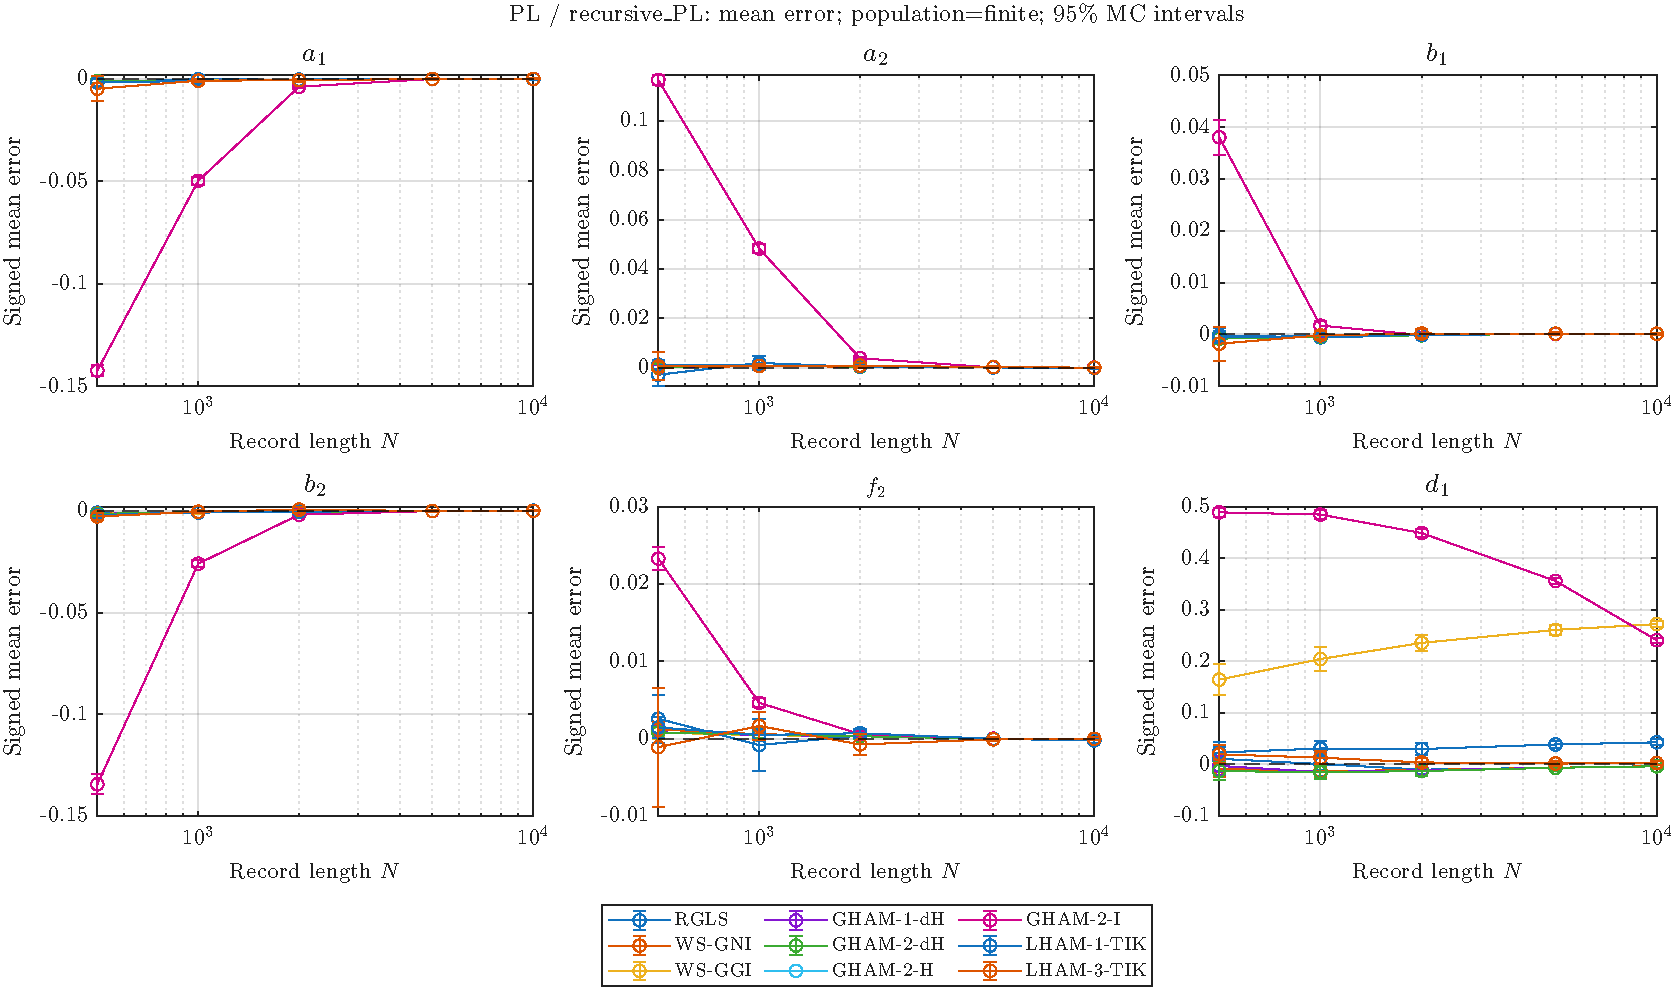
\includegraphics[width=.92\linewidth]{figs/record_length_bias_example_1_pl_recursive_PL.pdf}
\par\medskip
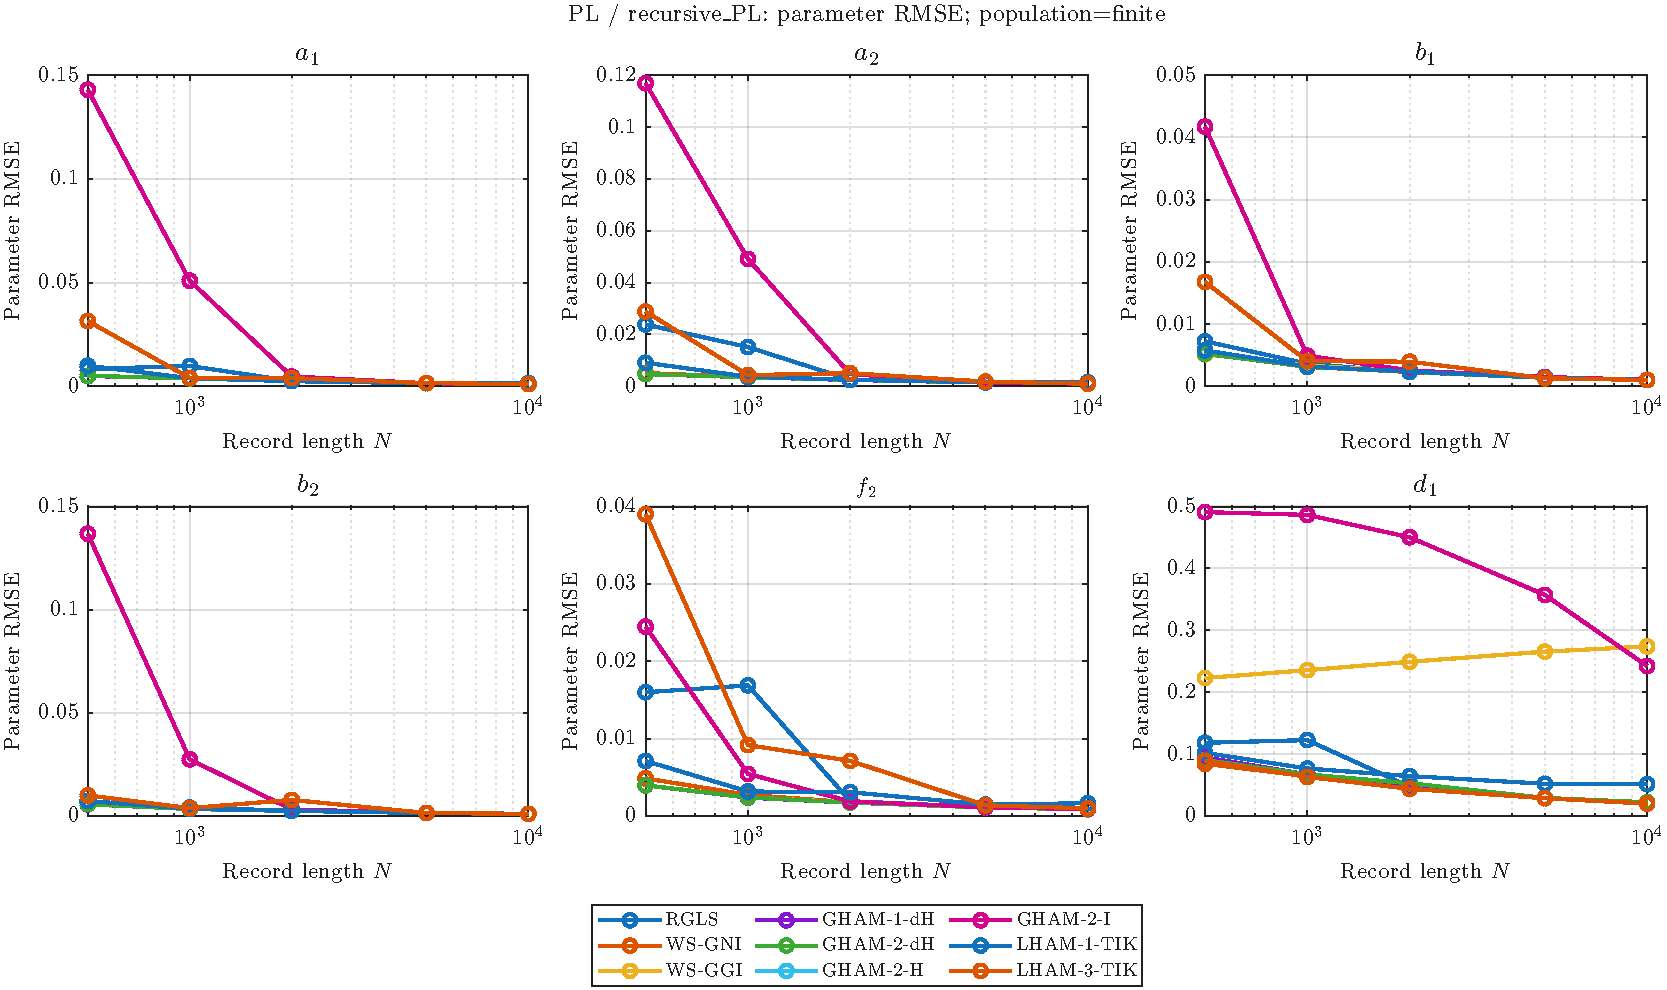
\includegraphics[width=.92\linewidth]{figs/record_length_rmse_example_1_pl_recursive_PL.pdf}
\caption{Example~1, PL: signed mean parameter errors with pointwise
$95\%$ Monte Carlo intervals (upper panel, linear vertical scale), and
parameter RMSEs (lower panel, logarithmic vertical scale). Bias ranges
show the last three record lengths; dashed segments indicate connections
to off-scale means, whose intervals are omitted.}
\label{fig:bias_ex1_pl}
\end{figure}

\begin{figure}[p]
\centering
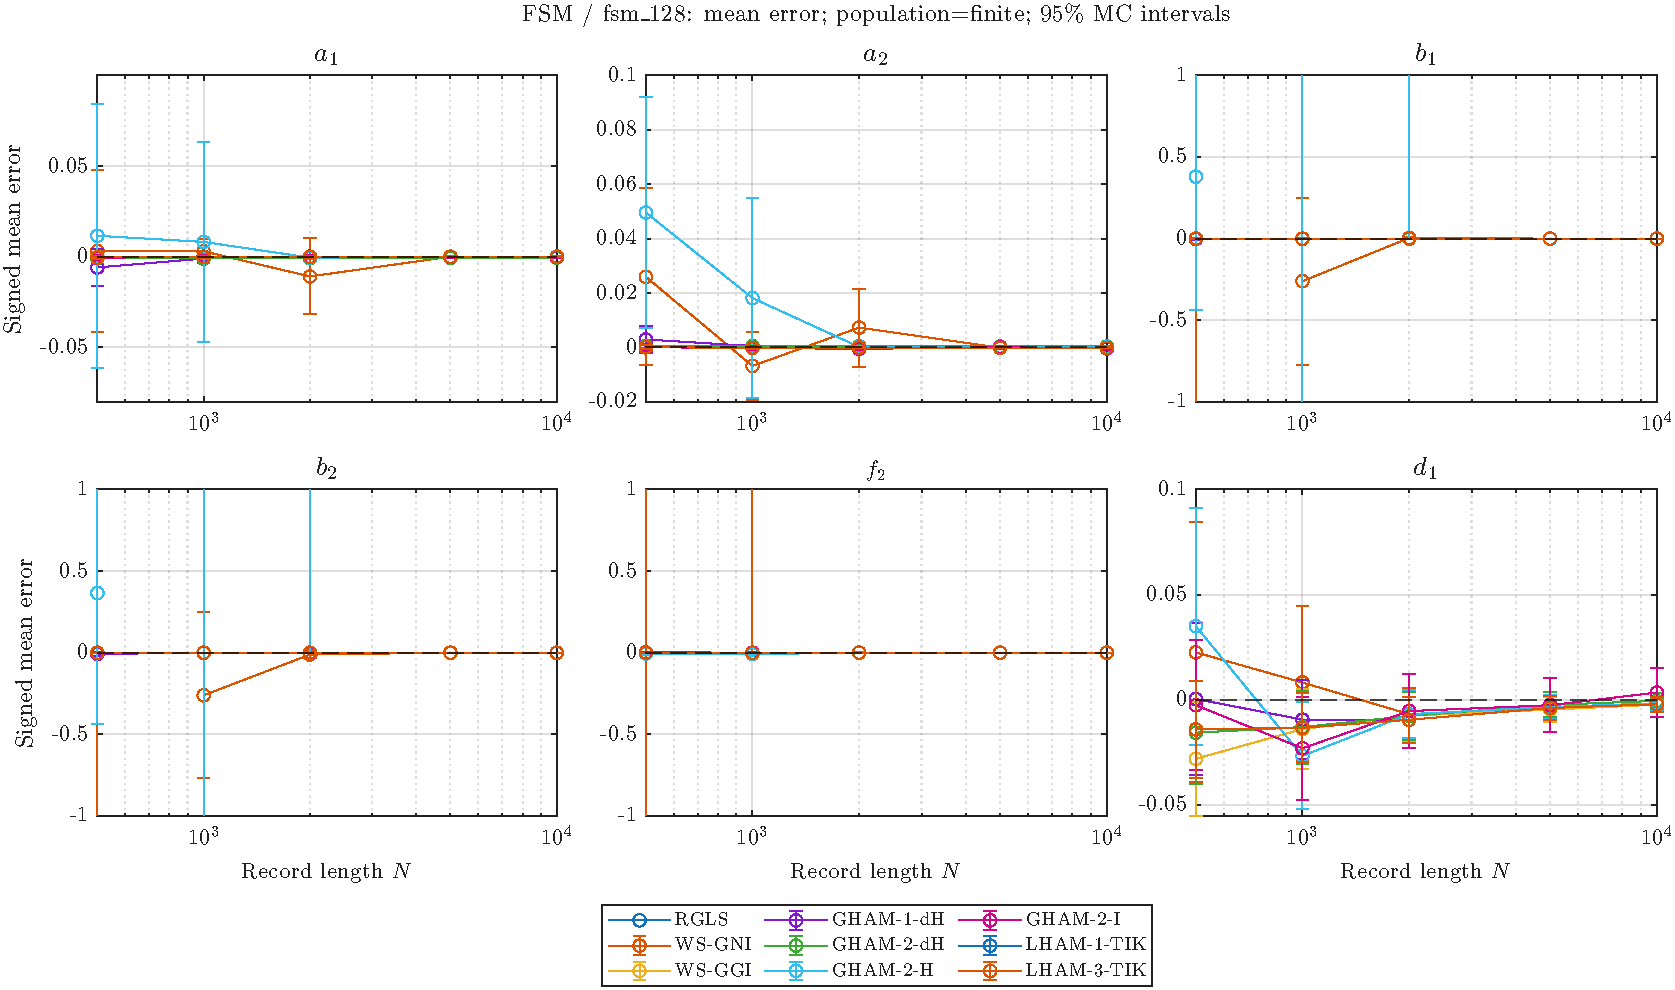
\includegraphics[width=.92\linewidth]{figs/record_length_bias_example_1_fsm_fsm_128.pdf}
\par\medskip
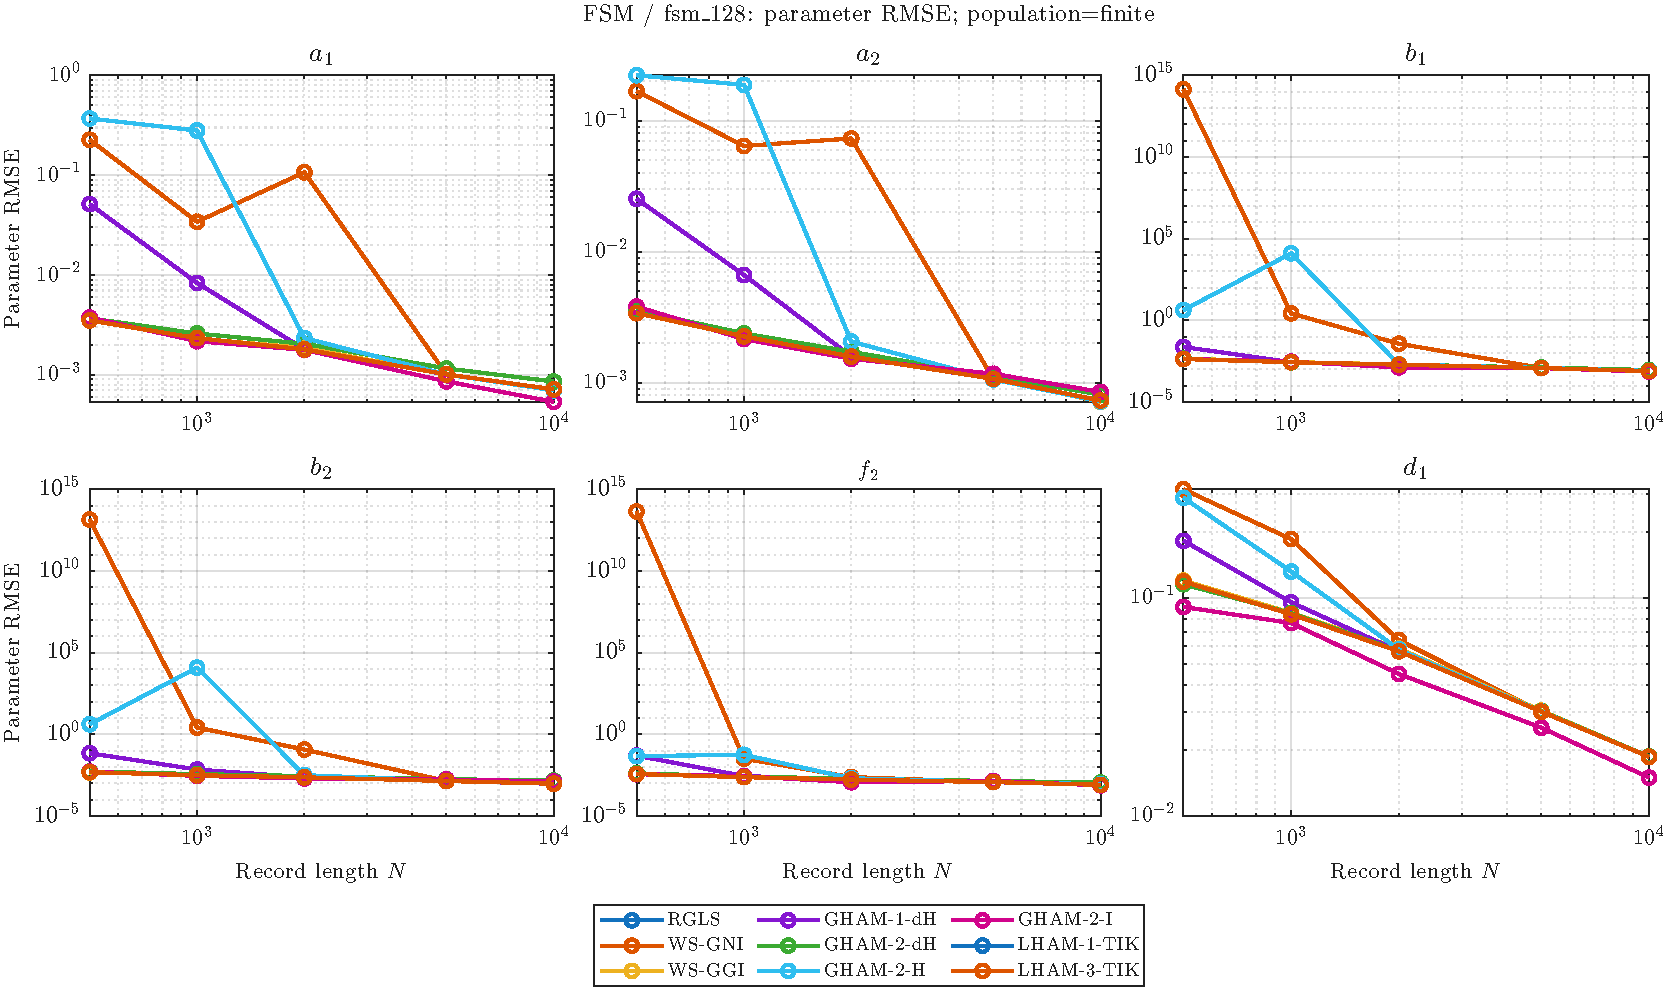
\includegraphics[width=.92\linewidth]{figs/record_length_rmse_example_1_fsm_fsm_128.pdf}
\caption{Example~1, FSM with $128$ coefficients and $1024$ frequency
samples: signed mean errors and pointwise $95\%$ Monte Carlo intervals
(upper panel, linear vertical scale), and RMSEs (lower panel,
logarithmic vertical scale). Display conventions follow
Fig.~\ref{fig:bias_ex1_pl}. Summaries exclude failed fits.}
\label{fig:bias_ex1_fsm128}
\end{figure}

\begin{figure}[p]
\centering
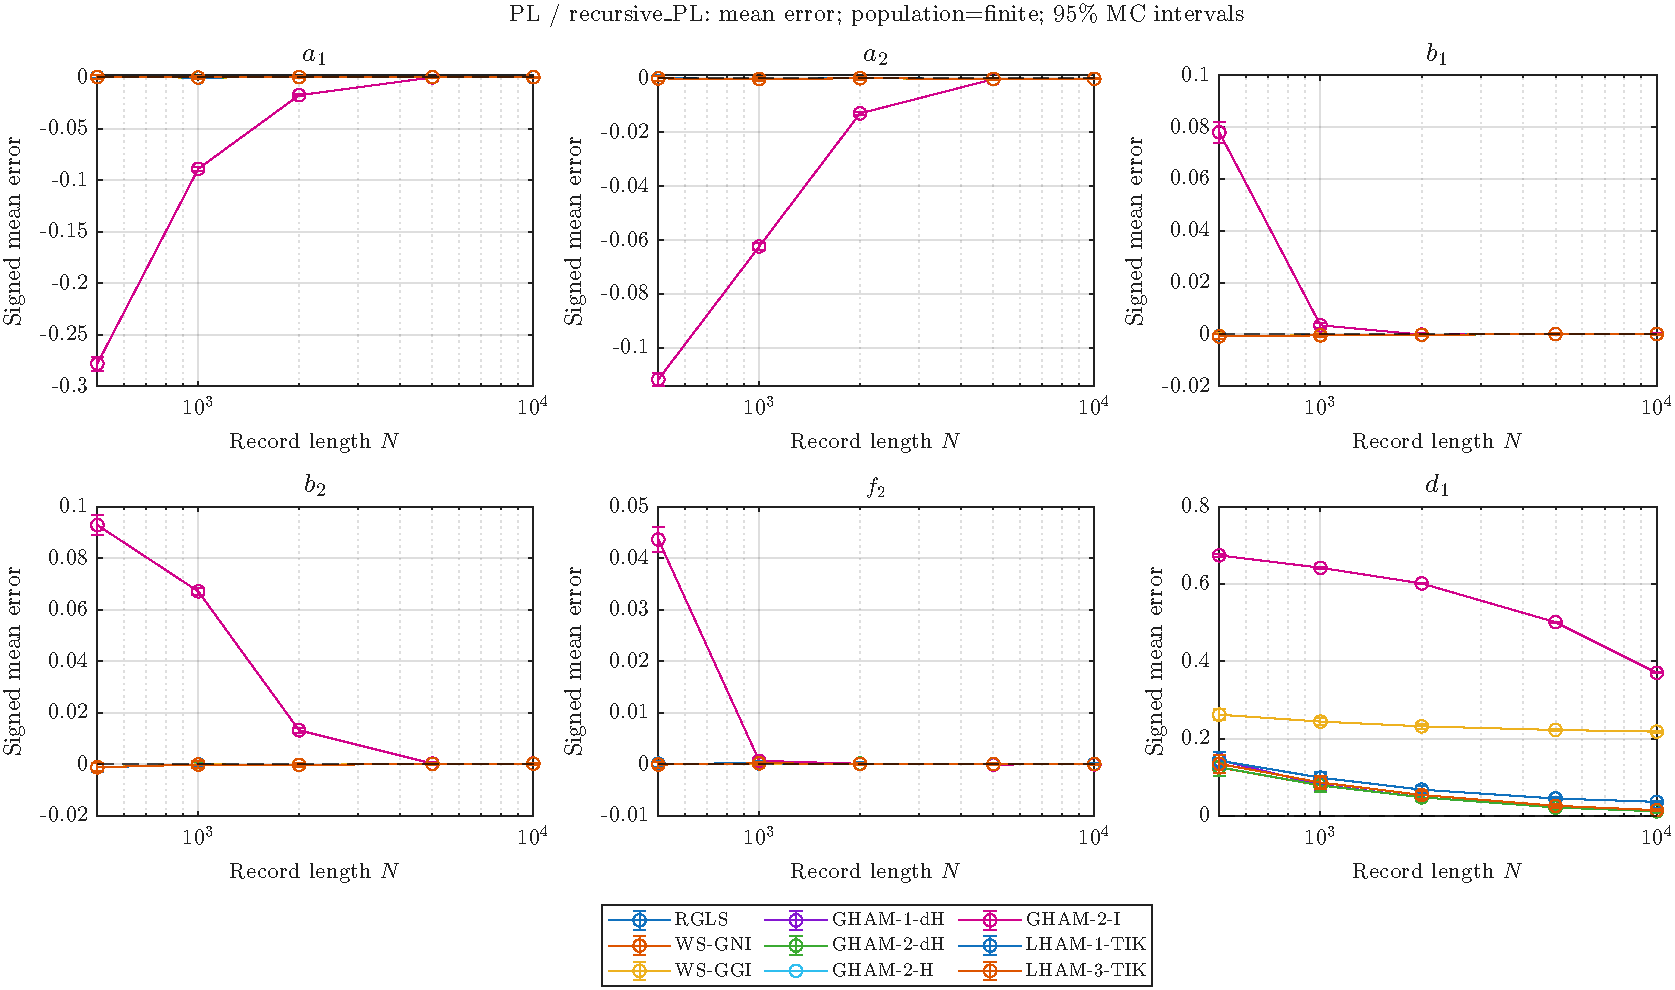
\includegraphics[width=.92\linewidth]{figs/record_length_bias_example_CSTR_pl_recursive_PL.pdf}
\par\medskip
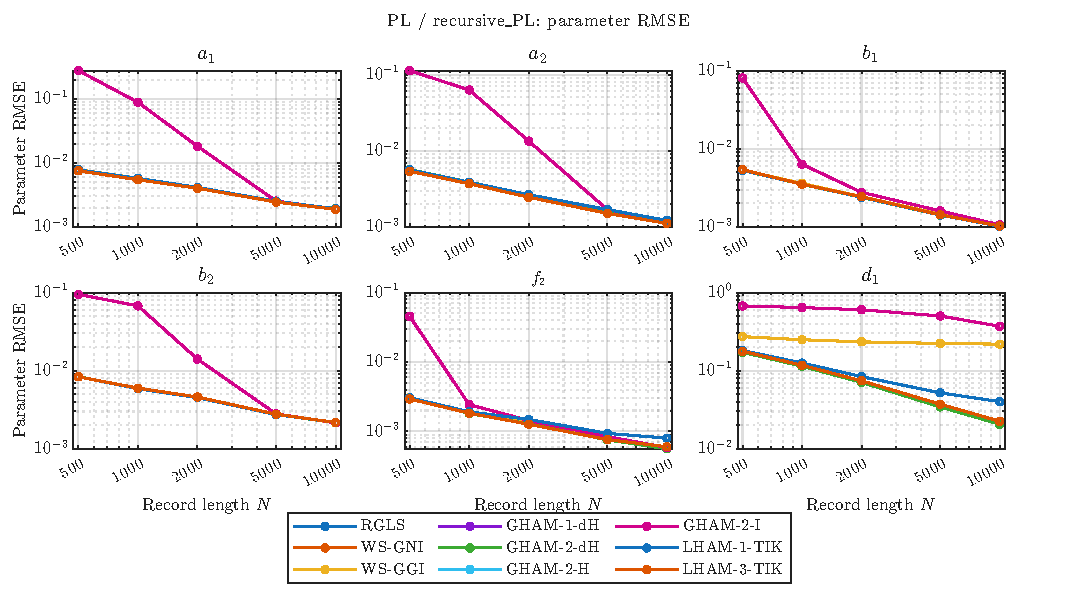
\includegraphics[width=.92\linewidth]{figs/record_length_rmse_example_CSTR_pl_recursive_PL.pdf}
\caption{CSTR, PL: signed mean parameter errors with pointwise
$95\%$ Monte Carlo intervals (upper panel, linear vertical scale), and
parameter RMSEs (lower panel, logarithmic vertical scale).
Display conventions follow Fig.~\ref{fig:bias_ex1_pl}.}
\label{fig:bias_cstr_pl}
\end{figure}

\begin{figure}[p]
\centering
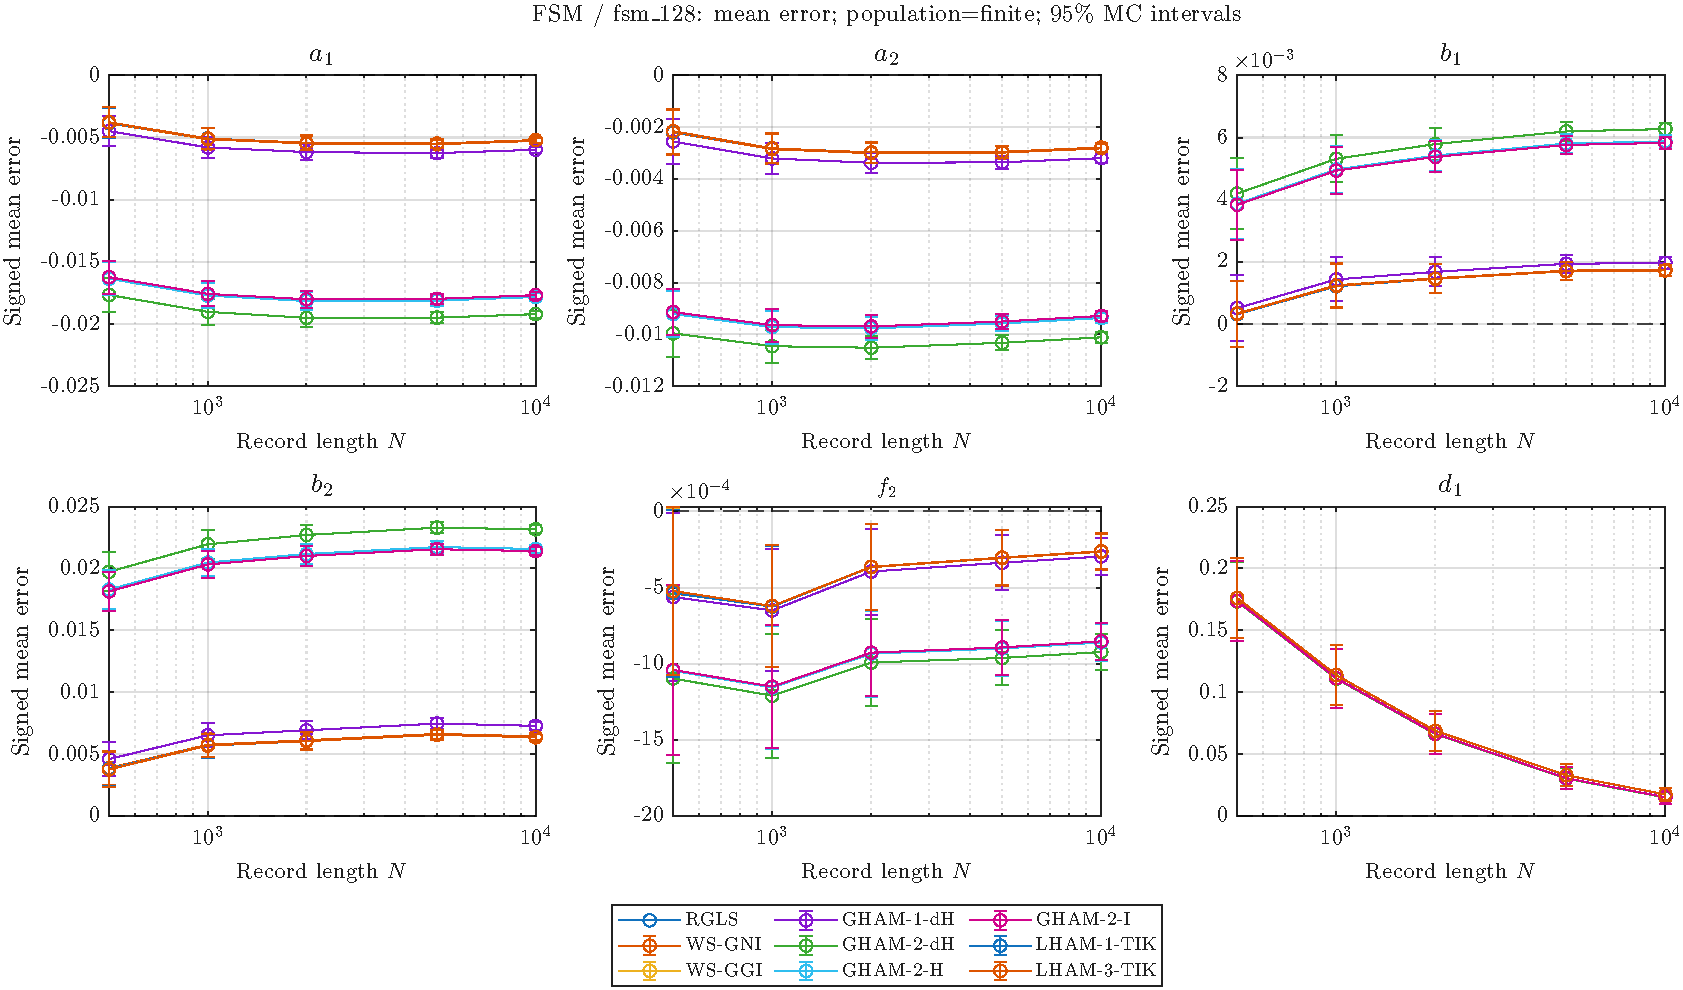
\includegraphics[width=.92\linewidth]{figs/record_length_bias_example_CSTR_fsm_fsm_128.pdf}
\par\medskip
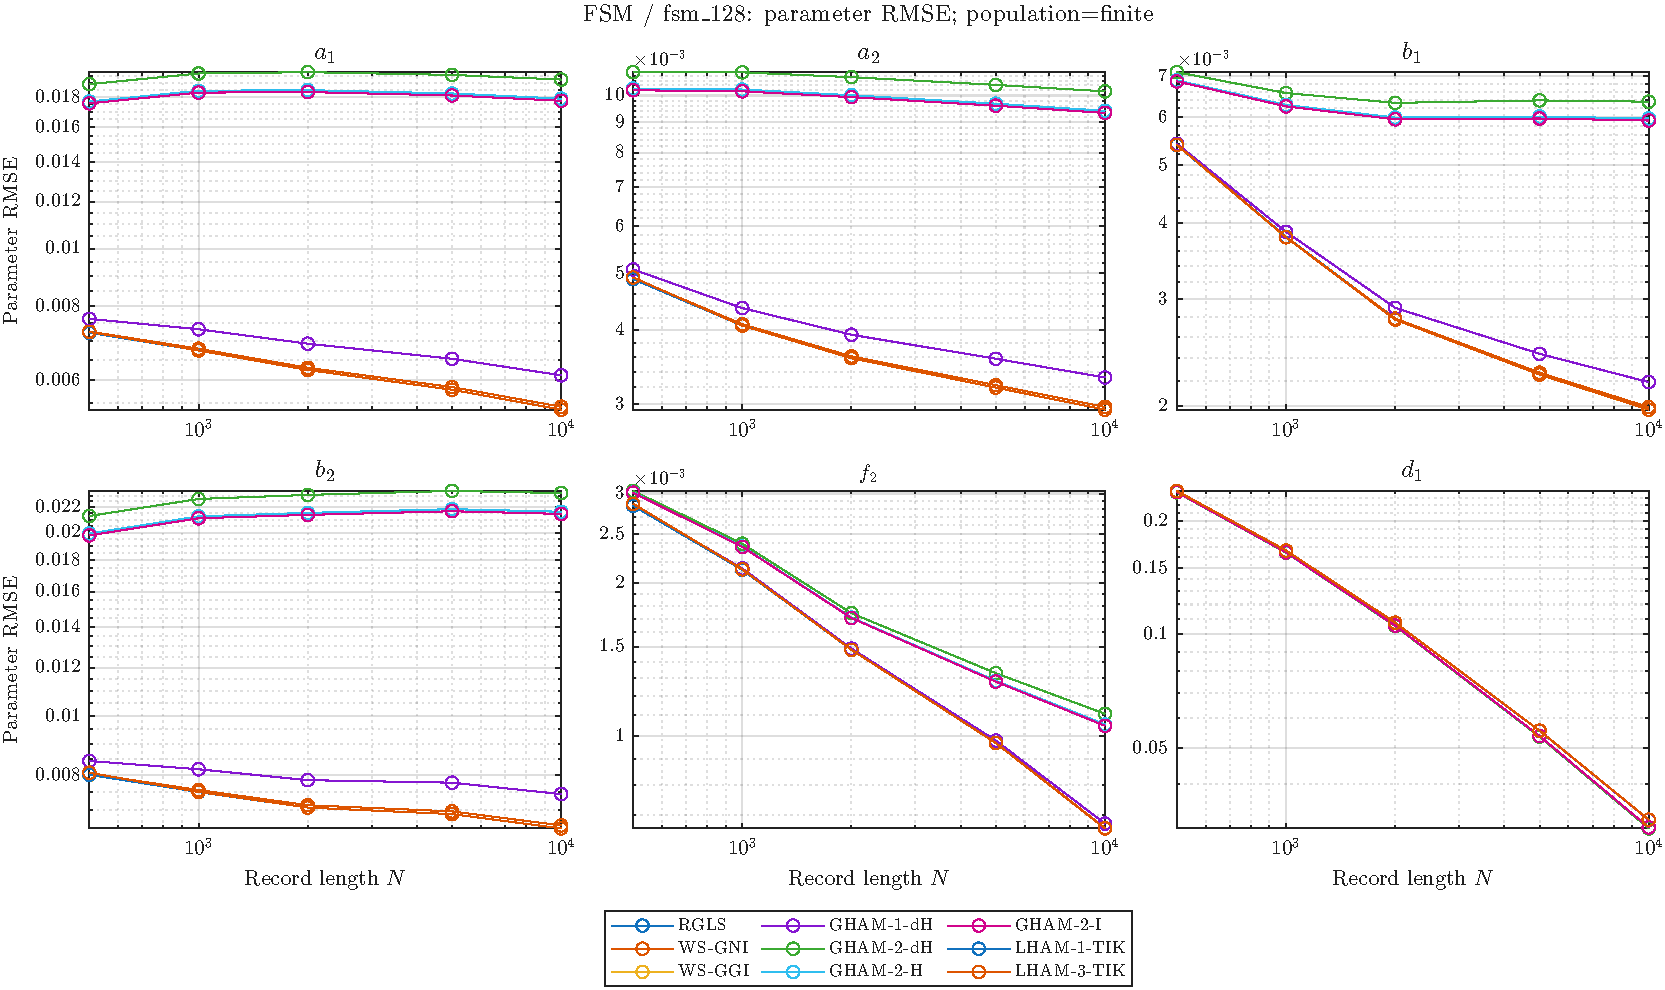
\includegraphics[width=.92\linewidth]{figs/record_length_rmse_example_CSTR_fsm_fsm_128.pdf}
\caption{CSTR, FSM with $128$ coefficients and $1024$ frequency samples:
signed mean errors and pointwise $95\%$ Monte Carlo intervals (upper
panel, linear vertical scale), and RMSEs (lower panel, logarithmic
vertical scale). Display conventions follow Fig.~\ref{fig:bias_ex1_pl}.}
\label{fig:bias_cstr_fsm128}
\end{figure}
